\documentclass[aps,pra,reprint,raggedbottom,superscriptaddress,amsmath,amssymb,longbibliography]{revtex4-2}
\usepackage[UTF8,scheme=plain]{ctex}
\usepackage{amsthm}
\usepackage{graphicx}
\usepackage[section]{placeins}
\usepackage[colorlinks=true,linkcolor=blue,citecolor=blue,urlcolor=blue]{hyperref}
\graphicspath{{assets/}}

\theoremstyle{definition}
\newtheorem{theorem}{定理}
\newtheorem{corollary}{推论}
\renewcommand{\proofname}{证明}
\renewcommand{\acknowledgmentsname}{致谢}
\renewcommand{\refname}{参考文献}
\renewcommand{\figurename}{FIG.}
\renewcommand{\abstractname}{摘要}
\newcommand{\dd}{\mathrm{d}}
\newcommand{\nvec}{\mathbf n}
\newcommand{\rvec}{\mathbf r}
\newcommand{\Rvec}{\mathbf R}
\newcommand{\vvec}{\mathbf v}
\newcommand{\ez}{\mathbf e_z}
\newcommand{\sigmavec}{\boldsymbol\sigma}

% 两种语言版本共用英文图注。
\newcommand{\shortcorpsecaption}{Short-CORPSE attaining the robust $\pi$-gate time.
(a) The saturated control segments have durations
$(\pi/3,5\pi/3,\pi/3)/\Omega$, with $u_y=0$.
(b) The planar error curve consists of three unit-radius circular arcs
in dimensionless coordinates $\Omega\mathbf r$. It returns to its
starting point with opposite initial and final tangents. Colors identify
the same control segments in both panels.}


\begin{document}

\title{固定时长量子比特 \texorpdfstring{$\pi$}{π} 门的最小一阶失谐残差}
\author{Tingyu Zhang}
\email{23300190021@m.fudan.edu.cn}
\affiliation{Department of Physics, Fudan University, Shanghai, China}
\author{Yan Cen}
\email[Corresponding author: ]{cenyan@fudan.edu.cn}
\affiliation{Department of Physics, Fudan University, Shanghai, China}

\begin{abstract}
抑制量子门的静态失谐误差需要延长控制时间，这也可能增加耗散损失。对于联合幅度受限、由任意可测横向控制驱动的完整量子比特 $\pi$ 门，我们确定了从最短标称门到最短一阶稳健门之间，每个时长所能达到的最小一阶失谐残差。全部取等控制仅由一个单轴三段脉冲族及其整体负号构成。该族连续连接矩形 $\pi$ 脉冲与 short-CORPSE，并确立了整个双轴控制类中完全抵消一阶失谐所需的最短时间 $7\pi/(3\Omega)$，其中 $\Omega$ 为最大驱动幅度。证明通过向时间中点的误差方向作几何投影得到下界，无需分类控制极值轨迹。所得边界同时确定了固定时长下，弱失谐引起的平均门不保真度二次系数的最小值。结合不依赖驱动的弱马尔可夫耗散，补偿程度的选择归结为对门时长的优化。在完全补偿附近略微缩短脉冲，节省的耗散与缩短量成正比，而新增的失谐代价仅为缩短量的二次项。因此，部分补偿能够比完全抵消一阶失谐得到更小的主导阶门误差。
\end{abstract}
\maketitle

\section{引言}

在共振时精确实现的量子门，仍可能随静态失谐发生一阶变化。复合脉冲通过将累积误差引向零来抑制这一变化，代价是更长的持续时间~\cite{cummins2000,cummins2003}。基本问题是：在给定时长下，残差能有多小，以及何时能够完全消除一阶误差。

门保真度易感性（gate fidelity susceptibility）以及稳健性与持续时间之间的权衡，已经在一般量子控制框架中得到表述~\cite{poggi2024}。相关的速度极限研究还考虑了给定误差子空间时，全控制下的稳健恒等操作~\cite{balada2026}。对于单量子比特门，数值优化已估计出实现指定稳健阶数所需的最短时间~\cite{cao2024}。在 Rydberg 门优化中，部分失谐补偿也成为一个实用的设计变量~\cite{bataille2026}。这些研究引出一个连续变化的问题：在精确实现标称门的条件下，每个允许时长对应的最小一阶失谐残差是多少？

所需时间取决于稳健性是针对指定输入态还是完整门。Van Damme 等报道了一阶失谐稳健布居反转的最短时间 $2\pi/\Omega$~\cite{vandamme2017}。对于完整量子比特 $\pi$ 门，已知 short-CORPSE 序列在 $7\pi/(3\Omega)$ 内完全消除一阶失谐响应~\cite{cummins2003}，且在三个基本脉冲构成的对称族内最优~\cite{kukita2022}。Pontryagin 分析研究了单轴控制下的选择性与稳健最短时间旋转~\cite{ansel2021}，并将 short-CORPSE 确定为时间最优候选解~\cite{kukita2024}；数值优化则给出一阶稳健 $X$ 门的时长接近 $2.33\pi/\Omega$~\cite{cao2024}。

在联合幅度受限、零失谐时精确实现完整量子比特 $\pi$ 门的条件下，本文研究以下问题：
\begin{enumerate}
\rightskip=0pt plus1fil
\item 每个给定时长的最小一阶失谐残差是多少？
\item 已知三段脉冲族能否在全部可测双轴控制中达到这一全局最小值？
\item 哪些控制能够达到残差下界？
\end{enumerate}

借助失谐误差的几何表示，可将该问题转化为曲率有界的路径问题~\cite{zeng2018,zeng2019,piliouras2026}。回到起点而切向反向的平面三弧轨迹出现在 Sigalotti 和 Chitour 的可控性构造中~\cite{sigalotti2006}，Kim 和 Cheong 则明确给出了其最短长度 $7\pi/3$~\cite{kim2013}。空间最短路径与可达性问题允许额外的非平面极值轨迹~\cite{sussmann1995,bae2025,bae2026,moser2022}。因此，平面构造本身不足以约束完整的双轴控制类。

本文的主要结果如下：
\begin{enumerate}
\rightskip=0pt plus1fil
\item 确定一阶失谐残差随时长变化的最小值，覆盖从最短矩形脉冲到 short-CORPSE 的整个区间。
\item 全部取等控制恰为上述单轴三段脉冲族及其整体负号；残差首次降为零的时长给出最短稳健时间 $7\pi/(3\Omega)$。
\item 采用 Schur 型切向比较~\cite{sullivan2008}，将误差方向投影到其在时间中点的取值，同时约束前后半段，无需分类全部控制极值轨迹。几何下界适用于任意不小于二的维数，其等号条件确定了全部最优曲线。
\item 将残差换算为弱失谐引起的平均门误差，并结合弱马尔可夫耗散的已知一阶效应~\cite{abad2022}，把两类误差共同作用下的最优补偿选择归结为同一三段脉冲族的持续时间优化。
\end{enumerate}

\section{控制模型与最小失谐残差}
\label{sec:model}

本章先明确可使用的控制，再将失谐的一阶响应表示为误差曲线的位移，从而把门误差的优化转化为几何问题。

我们只允许沿 $x$、$y$ 方向的横向驱动，没有独立的纵向控制。控制相位的改变仅改变此后的驱动方向，不施加额外的瞬时量子门；允许降低幅度、关闭驱动以及任意改变相位。失谐 $\delta$ 在一次门操作期间保持不变，控制函数不依赖这一未知失谐。取 $\hbar=1$，Pauli 矩阵的本征值为 $\pm1$，传播算符满足
\begin{equation}
 \begin{aligned}
 \dot U_\delta(t)&=-iH_\delta(t)U_\delta(t),\qquad U_\delta(0)=I,\\
 H_\delta(t)&=\frac{u_x(t)\sigma_x+u_y(t)\sigma_y+\delta\sigma_z}{2}.
 \end{aligned}
 \label{eq:dynamics}
\end{equation}
实控制函数 $u=(u_x,u_y)$ 可测，两个分量共同满足幅度约束
\begin{equation}
 u_x(t)^2+u_y(t)^2\le\Omega^2
 \quad\text{for almost every }t,
 \label{eq:disk}
\end{equation}
其中 $\Omega>0$ 为给定的最大驱动幅度。

令 $R_x(\theta)=\exp(-i\theta\sigma_x/2)$。零失谐时要求实现完整标称门
\begin{equation}
 U_0(T)=\pm R_x(\pi).
 \label{eq:target}
\end{equation}
正负号表示忽略整体相位。算符恒等式固定了它对每个输入态的作用。

为给出一阶失谐残差的几何表示，令 $\sigmavec=(\sigma_x,\sigma_y,\sigma_z)$，并定义
\begin{equation}
 \begin{aligned}
 \nvec(t)\cdot\sigmavec&=U_0(t)^\dagger\sigma_zU_0(t),\\
 \rvec(t)&=\int_0^t\nvec(t')\,\dd t'.
 \end{aligned}
 \label{eq:curve}
\end{equation}
这就是几何稳健控制中使用的误差曲线表示~\cite{zeng2019,piliouras2026}。对式~\eqref{eq:dynamics} 中的常值参数求变分，得到
\begin{equation}
 \left.\partial_\delta U_\delta(T)\right|_0
 =-\frac{i}{2}U_0(T)\,\rvec(T)\cdot\sigmavec.
 \label{eq:variation}
\end{equation}
因此，$\rvec(T)$ 记录失谐在整个门操作中累积的一阶作用：积分中的不同方向可以互相抵消，完全抵消等价于误差曲线回到起点，即 $\rvec(T)=0$。

\begin{figure}[!t]
\centering
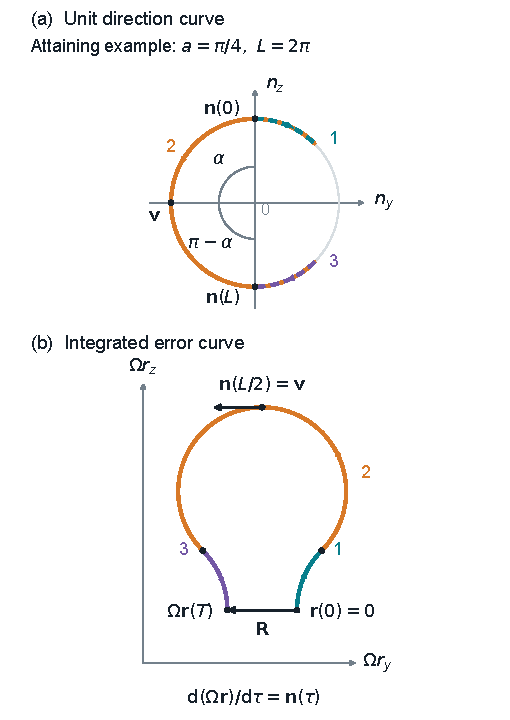
\includegraphics[width=\columnwidth]{residual_geometry.pdf}
\caption{\residualgeometrycaption}
\label{fig:geometry}
\end{figure}

酉共轭保持 Pauli 内积，故 $|\nvec|=1$，误差曲线具有单位速率 $|\dot\rvec|=1$。令 $\mathbf a_0,\mathbf b_0,\nvec$ 为分别共轭 $\sigma_x,\sigma_y,\sigma_z$ 所得的正交单位向量。对式~\eqref{eq:curve} 求导，其中的对易子给出
\begin{equation}
 \dot\nvec=u_x\mathbf b_0-u_y\mathbf a_0,\qquad
 |\dot\nvec|=\sqrt{u_x^2+u_y^2}\le\Omega
 \quad\text{a.e.}
 \label{eq:speed}
\end{equation}
用 $\ez$ 表示沿 $z$ 轴的单位向量，目标条件要求
\begin{equation}
 \nvec(0)=\ez,\qquad \nvec(T)=-\ez.
 \label{eq:antipodes}
\end{equation}
从球面一点到其反极点至少要转过 $\pi$，而转动速度不超过 $\Omega$，因而 $\Omega T\ge\pi$。对于有界可测控制，$U_0$ 和 $\nvec$ 为 Lipschitz 连续函数，$\rvec\in W^{2,\infty}$，各微分恒等式几乎处处成立。误差曲线可以自交，其曲率也可以在控制切换处不连续；这些情况都包含在上述控制类中。

定义 $L=\Omega T$，并以 $\tau=\Omega t$ 缩放时间，仍用 $\nvec$ 表示缩放后的方向。无量纲残差为
\begin{equation}
 \Rvec=\int_0^L\nvec(\tau)\,\dd\tau=\Omega\rvec(T).
 \label{eq:rescaled-error}
\end{equation}
对于初始 Bloch 向量为 $\ez$ 的态，式~\eqref{eq:variation} 表明，$\Rvec\parallel\ez$ 时一阶误差仅改变该态的整体相位；完整门的一阶抵消则要求 $\Rvec=0$。例如，文献~\cite{vandamme2017} 的两段稳健反转脉冲依次采用 $u_x=+\Omega,-\Omega$，持续时间为 $(3\pi/2,\pi/2)/\Omega$。这一脉冲实现标称门 $R_x(\pi)$，但其残差为 $\Rvec=-2\ez$，因此能够保护该输入态，却不能消除完整门的一阶失谐响应。

结合上述速度与端点条件，每个允许的完整量子门都给出一条绝对连续的单位向量曲线，其端点互为反极，速度不超过一。图~\ref{fig:geometry} 区分了两个几何对象：$\nvec$ 描述单位球面上的误差方向，积分曲线的切向量则为 $\nvec$，其端点位移就是残差 $\Rvec$。图中采用一条平面取等轨迹作示例，一般控制所产生的曲线无须共面。下面的定理确定完整门约束下的最小残差。




\begin{theorem}[最小失谐残差]
\label{thm:gate}
对每个固定的 $L\in[\pi,7\pi/3]$，在满足式~\eqref{eq:disk} 及完整标称门条件~\eqref{eq:target} 的全部控制中，
\begin{equation}
 \boxed{\min_u|\Rvec|=g(L),\qquad
 g(L)=4\cos\frac{L-\pi}{4}-2.}
 \label{eq:residual-minimum}
\end{equation}
除零测集上的改动外，全部取等控制均满足 $u_y=0$，且由 $u_x=+\Omega,-\Omega,+\Omega$ 三个相继的常值段或其整体负号构成，持续时间为
\begin{equation}
 \frac{1}{\Omega}(a,2a+\pi,a),\qquad
 a=\frac{L-\pi}{4}.
 \label{eq:family-durations}
\end{equation}
在 $L=\pi$ 时，外侧两段的持续时间为零。
\end{theorem}

最小值从 $2$（对应 $L=\pi$）降至 $L=7\pi/3$ 时的零。第~\ref{sec:midpoint} 章证明几何下界，第~\ref{sec:attainment} 章随后验证可达性并分类全部完整门等号情形。

\section{几何下界的证明}
\label{sec:midpoint}

本章把向量残差的估计化为一个标量积分。选取时间中点的误差方向作为投影轴后，曲线的每一半段既受到自身端点的约束，又必须及时到达这一中点。速度界限制了它能偏离投影轴多远，因此也限制了负投影能够抵消多少正投影。对这一距离约束积分，就得到残差下界。

\begin{theorem}[端点反极的球面曲线]
\label{thm:sphere}
设 $d\ge2$ 且 $\pi\le L\le7\pi/3$。对于每条绝对连续曲线 $\nvec:[0,L]\to S^{d-1}$，若 $|\nvec'|\le1$ 几乎处处成立，且 $\nvec(L)=-\nvec(0)$，令 $\vvec=\nvec(L/2)$ 及 $\Rvec=\int_0^L\nvec(\tau)\,\dd\tau$，则
\begin{equation}
 |\Rvec|\ge\vvec\cdot\Rvec\ge g(L)\ge0.
 \label{eq:sphere-bound}
\end{equation}
对于所述区间内的每个 $L$ 和每个 $d\ge2$，该界均可达到。
\end{theorem}

\begin{proof}
令 $c=L/2$，用 $d_S$ 表示球面测地距离，即两个单位向量的夹角，
\begin{equation*}
 d_S(\mathbf p,\mathbf q)=\arccos(\mathbf p\cdot\mathbf q).
\end{equation*}
曲线在 $[\tau_1,\tau_2]$ 内走过的球面弧长不超过 $|\tau_2-\tau_1|$，而两点间的最短球面距离不会大于这段弧长。因此，速度界给出
\begin{equation}
 d_S(\nvec(\tau_1),\nvec(\tau_2))\le|\tau_2-\tau_1|.
 \label{eq:lipschitz-sphere}
\end{equation}
若 $\alpha=d_S(\vvec,\nvec(0))$，则反极的另一端点到 $\vvec$ 的距离为 $\pi-\alpha$。前后半段各有时长 $c$，所以这两个距离都不能超过 $c$；再结合角度属于 $[0,\pi]$，得到
\begin{equation}
 \max(0,\pi-c)\le\alpha\le\min(\pi,c).
 \label{eq:feasible-alpha}
\end{equation}

将任一半段按从端点指向 $\vvec$ 的方向参数化，记为 $\mathbf m:[0,c]\to S^{d-1}$。前半段的初始距离为 $\beta=\alpha$，后半段反向参数化后为 $\beta=\pi-\alpha$。经过时间 $t$ 后，曲线到 $\vvec$ 的距离最多从 $\beta$ 增加到 $\beta+t$；同时，它还须在剩余时间 $c-t$ 内到达 $\vvec$，所以距离不能超过 $c-t$。球面上任意两点间的距离也不超过 $\pi$。合并这三个约束得到
\begin{equation}
 d_S(\vvec,\mathbf m(t))\le\min\{\beta+t,c-t,\pi\}.
 \label{eq:envelope}
\end{equation}
图~\ref{fig:envelope} 展示三个上界的下包络。若 $c+\beta\le2\pi$，两个斜线的交点不高于 $\pi$；若 $c+\beta>2\pi$，交点上方的尖顶被 $\pi$ 截成平台。这就是下面积分分成两支的原因。投影 $\vvec\cdot\mathbf m(t)$ 等于距离的余弦，余弦在 $[0,\pi]$ 上递减，因此距离的上界给出投影的下界。半段投影积分至少为
\begin{align}
 A(c,\beta)
 &:=\int_0^c\cos\bigl(\min\{\beta+t,c-t,\pi\}\bigr)\,\dd t
 \nonumber\\
 &=\begin{cases}
 2\sin\bigl((c+\beta)/2\bigr)-\sin\beta,
       &c+\beta\le2\pi,\\[1mm]
 2\pi-c-\beta-\sin\beta,
       &c+\beta\ge2\pi.
 \end{cases}
 \label{eq:A}
\end{align}

\begin{figure}[!htb]
\centering
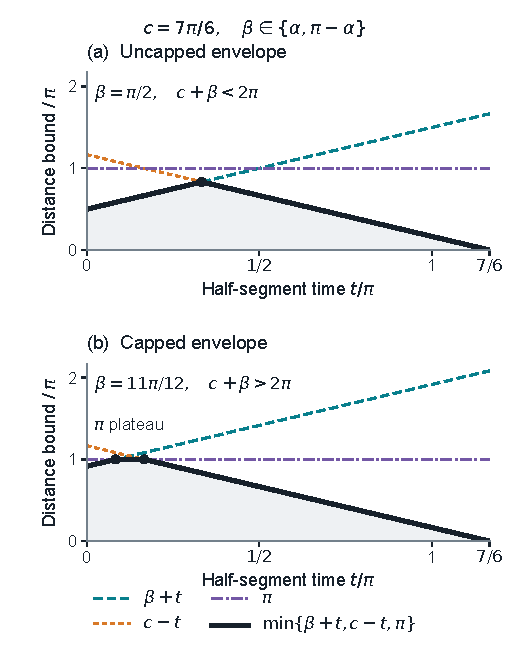
\includegraphics[width=\columnwidth]{midpoint_envelope.pdf}
\caption{\midpointenvelopecaption}
\label{fig:envelope}
\end{figure}

可行性条件 $0\le\beta\le\min(\pi,c)$ 保证两个仿射上界在非负时刻 $(c-\beta)/2$ 相交。在第二分支中，两者的最小值达到上限 $\pi$，并持续长度为 $c+\beta-2\pi$ 的区间。将两个半段相加，得到
\begin{equation}
 \vvec\cdot\Rvec\ge P(c,\alpha)
 :=A(c,\alpha)+A(c,\pi-\alpha).
 \label{eq:half-sum}
\end{equation}

下面比较不同中点取向 $\alpha$ 所允许的最小投影。若前后两个半段的包络都没有平台，即 $c+\alpha\le2\pi$ 且 $c+\pi-\alpha\le2\pi$，两项都采用式~\eqref{eq:A} 的第一支。令
\begin{equation*}
 K=\sin\left(\frac c2+\frac\pi4\right),\qquad
 x=\cos\left(\frac\alpha2-\frac\pi4\right).
\end{equation*}
此时 $1/2\le K\le1$、$1/\sqrt2\le x\le1$，且 $\sin\alpha=2x^2-1$。换元后，关于两段角度的三角表达式化为同一个二次多项式，
\begin{equation}
 P(c,\alpha)=4Kx-4x^2+2.
\end{equation}
它与所需下界之差可分解为
\begin{equation}
 P(c,\alpha)-(4K-2)=4(1-x)(1+x-K)\ge0.
 \label{eq:factor}
\end{equation}
第二个因子严格为正，故等号成立当且仅当 $\alpha=\pi/2$。当 $c\le\pi$ 时，每个可行的 $\alpha$ 都属于这一未截断情形。

若某一半段出现平台，由于交换 $\alpha$ 和 $\pi-\alpha$ 只会交换前后两项，可取 $\alpha\le\pi/2$。此时只有初始距离较大的后半段可能被截断，其条件是 $c+\pi-\alpha\ge2\pi$。因此只需处理区域
\begin{equation}
 \pi\le c\le7\pi/6,\qquad 0\le\alpha\le c-\pi\le\pi/6.
 \label{eq:cap-region}
\end{equation}
在此区域内，第一项未截断，且
\begin{equation}
 P(c,\alpha)=2\sin\frac{c+\alpha}{2}
              +\pi-c+\alpha-2\sin\alpha.
\end{equation}
由于 $(c+\alpha)/2\in[\pi/2,2\pi/3]$，
\begin{equation}
 \partial_\alpha P
 =\cos\frac{c+\alpha}{2}+1-2\cos\alpha
 \le1-\sqrt3<0.
 \label{eq:cap-monotonicity}
\end{equation}
因此，
\begin{equation*}
 P(c,\alpha)\ge P(c,c-\pi)>4K-2.
\end{equation*}严格不等式来自分支边界处的式~\eqref{eq:factor}，因为 $c-\pi\le\pi/6$ 不可能等于 $\pi/2$。结合两种情形可得
\begin{equation}
 P(c,\alpha)\ge4\sin(c/2+\pi/4)-2=g(L),
 \label{eq:scalar-bound}
\end{equation}
且只有在 $\alpha=\pi/2$ 时取等。由于 $|\vvec|=1$ 且 $g(L)\ge0$，式~\eqref{eq:sphere-bound} 得证。下面构造的平面脉冲族达到该界，并可嵌入任意 $d\ge2$ 维空间。
\end{proof}

等价地，该定理约束了每条长度为 $L$、曲率不超过一且两端切向相反的单位速率曲线的端点位移。在 $L=7\pi/3$ 时，最小位移首次降至零。

\section{下界的可达性与全部等号情形}
\label{sec:attainment}

本章构造达到下界的控制，并确定全部取等控制。几何比较只使用误差方向的端点和速度约束；要把几何最小值确认为量子门的最小值，还须验证构造实现了完整目标门，并用这一条件确定控制轴。

\FloatBarrier
\subsection{达到边界的三段脉冲族}

本节验证三段脉冲在给定区间的每个时长都实现标称门，并达到残差下界。

对于 $a=(L-\pi)/4\in[0,\pi/3]$，取 $u_y=0$ 及
\begin{equation}
 \frac{u_x}{\Omega}=q_a(\tau):=
 \begin{cases}
 +1,&0\le\tau<a,\\
 -1,&a\le\tau<3a+\pi,\\
 +1,&3a+\pi\le\tau\le4a+\pi.
 \end{cases}
 \label{eq:attaining-pulse}
\end{equation}
定义累积有符号转角
\begin{equation*}
 \phi(\tau)=\int_0^\tau q_a(\tau')\,\dd\tau'.
\end{equation*}
它在各段末端依次取值 $a,-a-\pi,-\pi$。零失谐哈密顿量彼此对易，因此
\begin{equation}
 U_0(T)=R_x(-\pi)=-R_x(\pi).
 \label{eq:attaining-gate}
\end{equation}
噪声方向为
\begin{equation}
 \nvec(\tau)=(0,\sin\phi(\tau),\cos\phi(\tau)).
 \label{eq:attaining-tangent}
\end{equation}
对三个区间积分得到
\begin{align}
 i\int_0^L e^{i\phi(\tau)}\,\dd\tau
 &=2e^{ia}-2e^{-i(a+\pi)}+e^{-i\pi}-1\nonumber\\
 &=4\cos a-2=g(L).
 \label{eq:attaining-error}
\end{align}
文献~\cite{kukita2024} 附录 D 的式 (D2) 已给出这一同轴三段族的积分。在单位驱动幅度、无量纲时间的约定下，所需形式为
\begin{equation*}
 I_c:=\int_0^L\cos\Theta(\tau)\,\dd\tau
 =4\sin\Theta_{\rm SB}-2\sin\frac{\theta_f}{2}.
\end{equation*}
其中 $\Theta$ 为移位后的累积转角，$\theta_f$ 为目标转角，$\Theta_{\rm SB}$ 为正的切换转角。在本文记号中，
\begin{equation*}
 \Theta=-\phi-\frac\pi2,\qquad
 \theta_f=\pi,\qquad \Theta_{\rm SB}=\frac\pi2+a.
\end{equation*}
$\Theta$ 依次从 $-\pi/2$ 走到 $-\Theta_{\rm SB}$、再到 $+\Theta_{\rm SB}$，最后回到 $+\pi/2$。因此该积分为 $I_c=4\cos a-2$，与式~\eqref{eq:attaining-error} 一致。

式~\eqref{eq:attaining-error} 给出 $\Rvec=-g(L)\mathbf e_y$；又因 $\phi(L/2)=-\pi/2$，有 $\vvec=-\mathbf e_y$。投影界和范数界均取等。控制整体取负后，残差范数不变，并满足标称目标的另一符号。

在 $a=\pi/3$ 时，该脉冲族为 short-CORPSE，误差曲线闭合，如图~\ref{fig:attainment} 所示。在 $a=0$ 时，它退化为单个矩形 $\pi$ 脉冲。因此，已知稳健构造和最短标称门是同一个全局取等脉冲族的两个端点。




\begin{figure}[!htb]
\centering
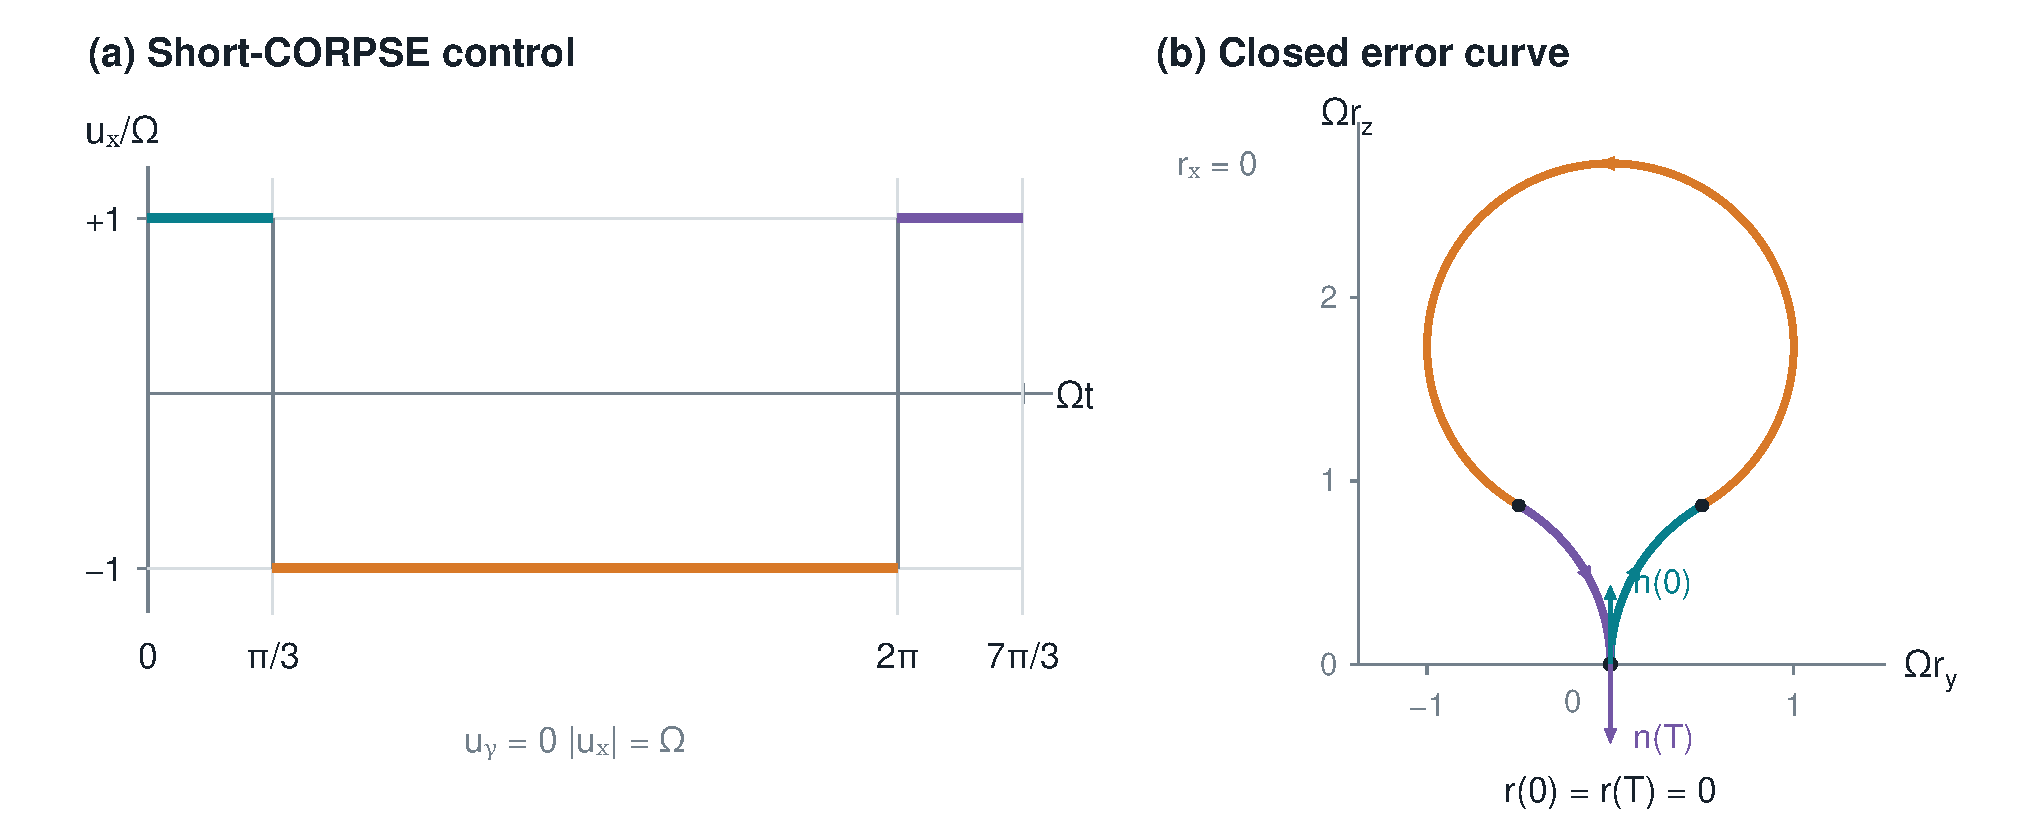
\includegraphics[width=\columnwidth]{short_corpse_geometry.pdf}
\caption{\shortcorpsecaption}
\label{fig:attainment}
\end{figure}

\subsection{几何刚性与控制唯一性}

本节沿下界证明逐步追踪等号条件：先确定中点取向，再确定曲线形状，最后用完整门条件选出上述两种控制。

假设 $|\Rvec|=g(L)$，则不等式链
\begin{equation}
 g(L)=|\Rvec|\ge\vvec\cdot\Rvec
 \ge P(c,\alpha)\ge g(L)
 \label{eq:equality-chain}
\end{equation}
中的每一步都必须取等，包括零点 $g(L)=0$ 的情形。于是 $\alpha=\pi/2$。两个半段投影积分中的逐点差值连续且非负，其总积分为零，因此这些差值恒为零。现在将各半段按从中点指向端点的方向参数化。其到 $\vvec$ 的距离必为
\begin{equation}
 \theta(\ell)=\min\{\ell,c+\pi/2-\ell\},\qquad 0\le\ell\le c.
 \label{eq:rigidity-angle}
\end{equation}
对 $\ell>0$，将半段曲线写成
\begin{equation}
 \mathbf m(\ell)=\cos\theta(\ell)\,\vvec
              +\sin\theta(\ell)\,\mathbf e(\ell),
\end{equation}
其中 $\mathbf e\perp\vvec$ 且 $|\mathbf e|=1$。由于 $0<\theta(\ell)\le c/2+\pi/4\le5\pi/6<\pi$，向量 $\mathbf e$ 在每个 $[\varepsilon,c]$ 上绝对连续。在该区间上几乎处处有
\begin{equation}
 |\mathbf m'|^2=(\theta')^2
       +\sin^2\theta\,|\mathbf e'|^2\le1.
 \label{eq:rigidity-speed}
\end{equation}
由 $|\theta'|=1$ 几乎处处成立可知，$\mathbf e$ 必为常向量。又因 $\theta(c)=\pi/2$，这两个常向量分别为 $\nvec(0)$ 和 $-\nvec(0)$。因此，两半曲线位于同一个大圆上，且形状恰好由式~\eqref{eq:attaining-pulse} 生成。在外侧两段消失的 $L=\pi$ 情形中，这一结论仍成立。

完整量子门条件固定了剩余的平面取向。给定 $\vvec\perp\ez$，令 $\mathbf a=\ez\times\vvec$。固定轴演化
\begin{equation*}
 U_a(t)=\exp\left[-\frac{i}{2}\phi(\Omega t)
                  \mathbf a\cdot\sigmavec\right]
\end{equation*}
生成该等号曲线。若另一横向演化 $U_0$ 生成同一个 $\nvec$，则 $W=U_0U_a^\dagger$ 与 $\sigma_z$ 对易，因而在其本征基中为对角矩阵。另一方面，
\begin{equation}
 \dot W=-iH_0W+iWH_a,
 \label{eq:lift-uniqueness}
\end{equation}
其中两个标称哈密顿量的对角元均为零。于是右端的对角元也均为零，而 $\dot W$ 为对角矩阵，因此 $\dot W=0$ 几乎处处成立。结合 $W(0)=I$，可得 $W=I$。最后，$U_a(T)=i\mathbf a\cdot\sigmavec$ 等于 $\pm R_x(\pi)$ 当且仅当 $\mathbf a=\pm\mathbf e_x$。故定理~\ref{thm:gate} 中的控制穷尽了全部取等情形。

结合中点下界和显式构造，定理~\ref{thm:gate} 的证明至此完成。残差界的首个零点随即给出最短稳健门时间。

\begin{corollary}[消除一阶误差的最短时间]
\label{cor:robust-time}
在满足完整门条件~\eqref{eq:target} 的允许控制中，若还要求 $\left.\partial_\delta U_\delta(T)\right|_{\delta=0}=0$，则最短持续时间为
\begin{equation}
 T_* = \frac{7\pi}{3\Omega}.
 \label{eq:robust-time}
\end{equation}
只有 short-CORPSE 及其整体负号达到这一时间，三段持续时间为 $(\pi/3,5\pi/3,\pi/3)/\Omega$。
\end{corollary}

\begin{proof}
式~\eqref{eq:variation} 使一阶误差抵消等价于 $\Rvec=0$。反极端点条件已要求 $L\ge\pi$，且 $g(L)>0$ 对 $\pi\le L<7\pi/3$ 成立。因此，定理~\ref{thm:gate} 排除了在 $7\pi/(3\Omega)$ 之前抵消误差的可能，并表明上述两种控制达到这一时间。其等号分类还给出它们在忽略零测集改动后的唯一性。
\end{proof}

\section{残差界的物理推论}
\label{sec:dissipation}

残差衡量传播算符对失谐的一阶响应，实际门性能则常用平均门保真度衡量。本章先建立两者的联系，再加入耗散损失，说明在有限相干时间内如何选择补偿程度以最小化总门误差。

\FloatBarrier
\subsection{失谐敏感度与平均门不保真度}

首先推导残差如何确定平均门不保真度中的失谐二次项。采用标准的平均门保真度，即对所有纯输入态的态保真度作均匀平均~\cite{bowdrey2002,nielsen2002}。对于固定的允许控制 $u=(u_x,u_y)$ 和无量纲失谐 $f=\delta/\Omega$，记
\begin{equation}
 \begin{aligned}
 V_f&=U_0(T)^\dagger U_{\Omega f}(T),\\
 F_{\rm avg}[u;f]&=\frac{|\operatorname{Tr}V_f|^2+2}{6},\\
 \chi[u]&=\lim_{f\to0}\frac{1-F_{\rm avg}[u;f]}{f^2}.
 \end{aligned}
 \label{eq:sensitivity}
\end{equation}
系数 $\chi$ 衡量小失谐引起的平均门误差，是门保真度易感性~\cite{poggi2024}在上述保真度及无量纲失谐约定下的表达。为明确归一化关系，记传播子保真度及其展开为
\begin{equation*}
 F_U=\frac{|\operatorname{Tr}V_f|^2}{4},\qquad
 1-F_U=\chi_U\delta^2+o(\delta^2),
\end{equation*}
两种保真度及敏感度之间满足
\begin{equation*}
 F_{\rm avg}=\frac{2F_U+1}{3},\qquad
 \chi=\frac{2\Omega^2}{3}\chi_U.
\end{equation*}

下面利用传播算符对失谐的一阶响应计算 $\chi$。相对传播算符属于 $SU(2)$，因而可写成
\begin{equation*}
 \begin{aligned}
 U_0(T)^\dagger U_\delta(T)
   &=w_\delta I-i\mathbf b_\delta\cdot\sigmavec,\\
 w_\delta^2+|\mathbf b_\delta|^2&=1,
 \end{aligned}
\end{equation*}
其中 $w_\delta$ 为实数，$\mathbf b_\delta$ 为实向量。式~\eqref{eq:variation} 确定其向量部分，
\begin{equation*}
 \mathbf b_\delta=\frac{\delta}{2}\rvec(T)+O(\delta^2).
\end{equation*}
将它代入保真度公式，得到
\begin{equation}
 \begin{aligned}
 1-F_{\rm avg}&=\frac23|\mathbf b_\delta|^2
 =\frac{\delta^2}{6}|\rvec(T)|^2+O(\delta^3),\\
 \chi[u]&=\frac{\Omega^2}{6}|\rvec(T)|^2.
 \end{aligned}
 \label{eq:chi-curve}
\end{equation}
这说明传播算符中关于失谐的一阶偏差对门不保真度产生二次贡献，且系数只取决于误差曲线端点位移的长度。因此，$\chi=0$ 等价于完整传播算符的一阶误差抵消，也等价于误差曲线闭合。

将定理~\ref{thm:gate} 应用于式~\eqref{eq:chi-curve}，得到
\begin{equation}
 \boxed{\chi_{\min}(L)=\frac{g(L)^2}{6}
 =\frac16\left[4\cos\frac{L-\pi}{4}-2\right]^2.}
 \label{eq:main}
\end{equation}
式~\eqref{eq:attaining-pulse} 中的控制及其整体负号在整个 $\pi\le L\le7\pi/3$ 上达到这一速度--敏感度边界。
最小值从 $\chi_{\min}(\pi)=2/3$（对应矩形 $\pi$ 脉冲）降至 short-CORPSE 对应的零。第二个可独立控制的横向轴不能进一步降低敏感度。例如，在 $L=2\pi$ 时，
\begin{equation*}
 \chi_{\min}(2\pi)
 =\frac{(2\sqrt2-2)^2}{6}\simeq0.11438.
\end{equation*}
此时门时长为完全消除一阶误差所需时间的 $6/7$，失谐敏感度已明显低于矩形脉冲。

\FloatBarrier
\subsection{弱耗散与联合误差预算}

本节推导耗散的一阶损失，并在明确的弱噪声极限下将其与静态失谐贡献相结合。
考虑对称、零均值的准静态失谐分布，以及独立且不依赖驱动的马尔可夫弛豫和退相位，采用标准 Lindblad 形式~\cite{gorini1976,lindblad1976}，
\begin{equation}
 \dot\rho=-i[H_\delta,\rho]
 +\Gamma_1\mathcal D[\sigma_-]\rho
 +\frac{\Gamma_\phi}{2}\mathcal D[\sigma_z]\rho,
 \label{eq:lindblad}
\end{equation}
这里的耗散子及跃迁算符定义为
\begin{equation*}
 \begin{aligned}
 \mathcal D[A]\rho
   &=A\rho A^\dagger-\frac12\{A^\dagger A,\rho\},\\
 \sigma_-&=\frac{\sigma_x-i\sigma_y}{2}.
 \end{aligned}
\end{equation*}
在此约定下，$\Gamma_\phi$ 为纯退相位速率，横向衰减速率为 $\Gamma_2=\Gamma_1/2+\Gamma_\phi$。这些速率均不依赖驱动。对于这一开放系统动力学，$F_{\rm avg}$ 表示该量子通道相对于同一标称酉门的平均态保真度。

先在 $\delta=0$ 时单独计算耗散贡献。Bloch 动力学齐次部分的阻尼矩阵为
\begin{equation*}
 D=\operatorname{diag}(-\Gamma_2,-\Gamma_2,-\Gamma_1).
\end{equation*}
令 $O_0(t)$ 表示理想 Bloch 旋转，$\Gamma=\Gamma_1+\Gamma_\phi$。在理想旋转参考系中，通道的齐次部分为
\begin{equation*}
 M=I+\int_0^T O_0(t)^{\mathsf T}D O_0(t)\,\dd t
       +O((\Gamma T)^2).
\end{equation*}
对仿射 Bloch 通道，平均门保真度只需其齐次矩阵的迹~\cite{bowdrey2002,nielsen2002}：
\begin{equation*}
 \mathbf q\mapsto M\mathbf q+\mathbf c,
 \qquad F_{\rm avg}=\frac12+\frac{\operatorname{Tr}M}{6}.
\end{equation*}
这里以恒等通道为参考，平移项 $\mathbf c$ 在所有输入方向上的平均为零。旋转共轭又不改变 $D$ 的迹，因此一阶迹修正为 $T\operatorname{Tr}D$，得到
\begin{equation}
 1-F_{\rm avg}
 =\frac{\Gamma_1+\Gamma_\phi}{3}T+O((\Gamma T)^2),
 \qquad\Gamma=\Gamma_1+\Gamma_\phi.
 \label{eq:weak-dissipation}
\end{equation}



这就是普适一阶保真度损失~\cite{abad2022}在单比特情形下的表达。其物理含义是：在这些假设下，驱动只能旋转耗散作用的方向，不能改变其对平均门保真度的一阶损失率。因此，同样长的脉冲具有相同的主导耗散代价，减小该代价需要缩短时间。

现在把两类误差放在同一弱噪声尺度下比较。固定控制、有限时长和 $\gamma_j$，令
\begin{equation*}
 \delta=\eta\xi,\qquad
 \Gamma_j=\eta^2\gamma_j\quad(j=1,\phi),\qquad \eta\to0.
\end{equation*}
其中 $\xi$ 的分布对称且具有有限四阶矩。这样，失谐的二次贡献和耗散的一次贡献同为 $\eta^2$ 阶。定义
\begin{equation}
 s^2=\frac{\operatorname{Var}(\delta)}{\Omega^2},
 \qquad
 \kappa=\frac{\Gamma_1+\Gamma_\phi}{3\Omega}.
 \label{eq:noise-parameters}
\end{equation}
在联合展开中，对称分布使所有关于 $\delta$ 的奇次项平均为零，其中包括 $\delta\Gamma_j$ 型的三阶混合项。剩余的失谐四次项、失谐二次项与耗散的混合项以及耗散二次项均从 $\eta^4$ 阶开始；有限四阶矩保证可对余项取平均。结合静态误差展开和式~\eqref{eq:weak-dissipation}，得到
\begin{equation}
 \mathbb E[1-F_{\rm avg}]
 =s^2\chi[u]+\kappa L+O(\eta^4).
 \label{eq:combined-expansion}
\end{equation}
对于达到边界的单轴脉冲族，还可直接看到其酉演化保真度为何为失谐的偶函数：
\begin{equation*}
 H_{-\delta}=\sigma_xH_\delta\sigma_x,
\end{equation*}
这一共轭关系同时保持初始条件和标称目标，故失谐取反不改变相对传播算符的迹。一般双轴控制的奇次项则由上述分布对称性消去。

$s^2\chi[u]+\kappa L$ 是平均门不保真度的主导项，系数由失谐方差与衰减速率确定。主导阶相干与耗散损失相加的处理见于弱耗散展开~\cite{abad2022}及短时与稳健 Rydberg 门的比较~\cite{fromonteil2023}。固定 $L\in[\pi,7\pi/3]$ 时，对全部允许波形最小化得到
\begin{equation}
 \boxed{\mathcal E_{\min}(L)=s^2\chi_{\min}(L)+\kappa L.}
 \label{eq:budget}
\end{equation}
脉冲族~\eqref{eq:attaining-pulse} 达到该值。固定时长时，耗散项对所有波形相同，因此使残差最小的控制也使联合主导误差最小。接下来只需决定是否值得延长这一脉冲来换取更强的失谐补偿。



\FloatBarrier
\subsection{平衡失谐抑制与耗散}

完全抵消一阶失谐需要最长的补偿脉冲，但量子比特在这段时间内持续发生耗散。如果耗散损失超过进一步抵消失谐的收益，提前结束脉冲、保留少量失谐残差会更有利。本节用式~\eqref{eq:budget} 比较这两种代价，确定最佳持续时间；由于每个时长的最优波形已经确定，这一比较覆盖全部允许控制。

对于 $\kappa>0$，持续时间 $L>7\pi/3$ 不可能改善主导阶误差预算：仅其耗散项就已超过稳健端点的预算 $\kappa(7\pi/3)$。因此，选择最佳主导阶工作点无需知道更长持续时间下的敏感度边界。

对于 $s^2>0$，定义两类噪声的相对权重及归一化预算，
\begin{equation*}
 \lambda=\frac{\kappa}{s^2},\qquad
 J(L)=\frac{\mathcal E_{\min}(L)}{s^2}
     =\chi_{\min}(L)+\lambda L.
\end{equation*}
$\lambda$ 较小时，失谐抑制更重要；$\lambda$ 较大时，额外的门时间代价更高。内部驻点要求延长门时间带来的两项边际变化互相抵消，即
\begin{equation}
 J'(L)=\lambda-\frac{g(L)}{3}\sin\frac{L-\pi}{4}=0.
 \label{eq:working-point}
\end{equation}
全局最优时长可以进一步明确确定。令 $a=(L-\pi)/4\in[0,\pi/3]$，并记
\begin{equation}
 p(a)=\frac23(2\cos a-1)\sin a.
 \label{eq:budget-slope}
\end{equation}
由于 $p'(a)=\frac23(4\cos^2a-\cos a-2)$，$p$ 在 $a_m=\arccos[(1+\sqrt{33})/8]$ 之前递增，之后递减至零。对于 $\lambda>0$，矩形端点始终是局部极小值，稳健端点则不是极小值；方程 $p(a)=\lambda$ 的内部根中，只有较大根可能给出极小值。在这样的驻点处，相对矩形脉冲的预算差为
\begin{equation*}
 D(a)=\chi_{\min}(\pi+4a)+4a p(a)-\frac23.
\end{equation*}
由 $D'(a)=4a p'(a)$、$D(0)=0$ 和 $D(\pi/3)=-2/3$ 可知，$D$ 在 $(a_m,\pi/3)$ 上恰有一个零点 $a_c$。其满足
\begin{equation}
 a_c(2\cos a_c-1)\sin a_c=\cos a_c(1-\cos a_c).
 \label{eq:budget-transition}
\end{equation}
对应的临界噪声比和时长为
\begin{equation}
 \begin{aligned}
 \lambda_c&=p(a_c)\simeq0.17625857,\\
 L_c&=\pi+4a_c\simeq2.04725676\pi.
 \end{aligned}
 \label{eq:budget-critical}
\end{equation}
当 $0<\lambda<\lambda_c$ 时，唯一最优时长对应上述内部极小值；在 $\lambda=\lambda_c$ 时，$L=\pi$ 与 $L=L_c$ 并列为全局最小点；当 $\lambda>\lambda_c$ 时，唯一最优时长为 $L=\pi$，由矩形脉冲实现。因此，尽管脉冲族中的补偿程度连续可调，最优时长仍会在这一阈值处跳至 $\pi$。

图~\ref{fig:frontier} 展示了敏感度边界及选择中间补偿程度的收益。为与两个端点脉冲中较优者比较，对 $\lambda>0$ 定义
\begin{equation}
 \begin{aligned}
 B(\lambda)&=\min\left\{\frac23+\pi\lambda,\frac{7\pi}{3}\lambda\right\},\\
 G(\lambda)&=1-\frac{\min_{\pi\le L\le7\pi/3}J(L)}{B(\lambda)}.
 \end{aligned}
 \label{eq:relative-gain}
\end{equation}
两端点预算在 $\lambda_0=1/(2\pi)$ 相交。固定 $L$ 时，比值 $J(L)/B(\lambda)$ 在交点之前随 $\lambda$ 不增，之后不减：第一支中的失谐贡献与 $1/\lambda$ 成正比，而第二支导数的符号由 $(2/3)L-\pi\chi_{\min}(L)\ge0$ 决定，这里用到了 $L\ge\pi$ 和 $0\le\chi_{\min}\le2/3$。对 $L$ 取最小值仍保持这两侧的单调性，故最大收益出现在 $\lambda_0$；最优内部脉冲对应的严格不等式又保证这一正的最大值唯一。数值上，
\begin{equation}
 \begin{aligned}
 G(\lambda_0)&\simeq4.91070\%,\\
 L_{\rm opt}(\lambda_0)&\simeq2.08454\pi.
 \end{aligned}
 \label{eq:maximum-gain}
\end{equation}
此时两个端点预算均为 $7/6$，上述数值就是相对较优端点的最大主导阶收益。部分补偿保留了大部分失谐抑制能力，同时缩短了耗散作用的时间。


\begin{figure}[!htb]
\centering
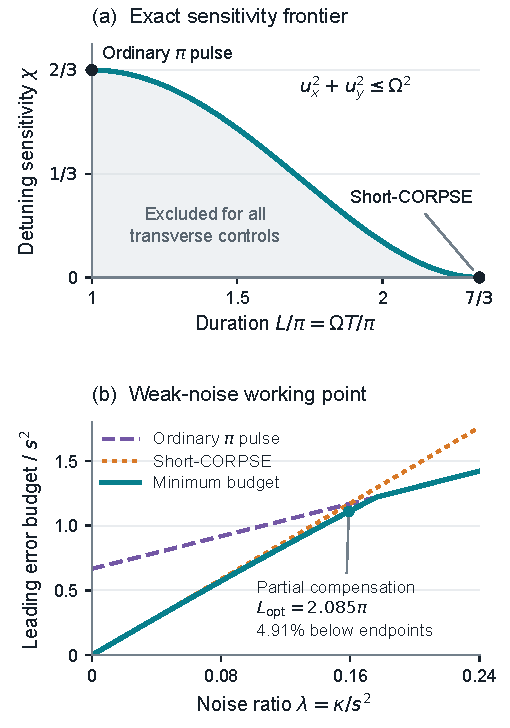
\includegraphics[width=\columnwidth]{frontier_working_point.pdf}
\caption{\frontiercaption}
\label{fig:frontier}
\end{figure}


在稳健端点 $L_*=7\pi/3$ 附近，部分补偿的优势尤其直观。对于 $h=L_*-L\downarrow0$，
\begin{equation}
 \chi_{\min}(L_*-h)=\frac{h^2}{8}+O(h^3),
 \label{eq:near-robust}
\end{equation}
因此
\begin{equation}
 \mathcal E_{\min}(L_*-h)-\mathcal E_{\min}(L_*)
 =-\kappa h+\frac{s^2h^2}{8}+O(s^2h^3).
 \label{eq:compensation-cost}
\end{equation}
式~\eqref{eq:compensation-cost} 解释了部分补偿的优势：从完全补偿端点略微缩短时间，节省的耗散为 $\kappa h$，新产生的失谐损失却只有 $s^2h^2/8$。对于足够小的正 $h$，线性收益总会超过二次代价。因此，只要耗散率为正，完全补偿就不会使主导阶误差最小。

当 $\lambda\to0^+$ 时，平衡这两项的导数得到最优缩短量
\begin{equation*}
 h=4\lambda+O(\lambda^2),\qquad \lambda\to0^+.
\end{equation*}
式~\eqref{eq:combined-expansion} 说明这一选择的精度：当前比较保留 $\eta^2$ 阶门误差，而高阶修正从 $\eta^4$ 阶开始。因而在噪声趋弱、两种脉冲的主导误差存在非零差别时，这一比较决定了实际误差的先后次序；若主导项相同或噪声不再足够弱，就需保留更高阶项来判断。

\section{讨论}
\label{sec:discussion}

最小残差曲线把两个通常分开讨论的问题连接起来：在给定时间内能抵消多少失谐误差，以及完全抵消至少需要多长时间。它的非零部分给出有限时间下无法消除的残差，首个零点则给出最短稳健时间。由于最短标称门的时长为 $\pi/\Omega$，一阶完全补偿需要把时间增加到其 $7/3$ 倍；中间的每一点说明提前结束脉冲必须承担多少误差。这使“是否稳健”的二元要求变成可定量选择的补偿程度。

从数学上看，中点投影将对任意空间曲线的优化化为两个半段距离包络的比较。下界在更大的曲线类中成立，因而无需假设最优控制存在、预设平面性或分类控制极值轨迹。等号分析又从同一个估计中恢复最优曲线：径向距离的变化已经用满速度限额，不再允许额外的侧向运动，因此两半曲线必须共面。这解释了为何增加横向控制方向或切换次数不能突破残差界。反极端点使两个初始距离之和固定为 $\pi$，是这一论证的关键；其他目标转角须重新处理端点及完整门约束。

本文证明了达到残差界的三段脉冲族给出全部允许双轴控制的全局最小值，并穷尽取等控制。这里完整门条件也不可省略：误差方向曲线只约束一个旋转轴的像，完整传播算符进一步固定剩余的平面取向。结果因此针对任意输入态的同一个目标门，而不只是把某个指定态翻转。

保真度关系给这一几何结论以直接的物理读出。累积误差方向决定传播算符对小失谐的线性偏离，其长度的平方决定平均门不保真度的二次系数。于是，残差最小值同时给出可达到的最小失谐敏感度；几何上闭合与否，对应这一领先误差项是否消失。

加入不依赖驱动的弱耗散后，补偿程度取决于两类误差的竞争。固定时长的耗散损失不随波形改变，所以整类控制的优化仍由同一三段脉冲族实现，只须选择其持续时间。完全补偿附近的线性耗散节省与二次失谐代价说明，为何少量残差可以换来更小的总门误差。

实际采用这一脉冲族时，还需考虑失谐模型之外的控制误差。同轴三段在零失谐时具有净转角 $-\pi$（整体取负时为 $+\pi$），共同的乘性幅度误差会直接改变这一转角，因此该族仍对幅度误差一阶敏感。部分或完全补偿的取等脉冲还依赖瞬时反向；有限带宽或切换速率进一步限制可行控制，本文的残差界仍成立，但原三段族未必能够达到它。若耗散速率随驱动改变，耗散损失也须随波形重新计算，此时失谐残差最小的控制未必使总误差最小；非准静态噪声同样需要调整误差模型。

\section{结论}
\label{sec:conclusion}

对于联合横向幅度受限的完整标称量子比特 $\pi$ 门，我们确定了从 $\pi/\Omega$ 到 $7\pi/(3\Omega)$ 的每个时长下的一阶失谐残差最小值。令 $L=\Omega T\in[\pi,7\pi/3]$，中点投影给出覆盖全部允许可测控制的下界
\begin{equation*}
 |\Rvec|\ge g(L)=4\cos\frac{L-\pi}{4}-2.
\end{equation*}
只有所述单轴三段脉冲族及其整体负号能够达到该界。边界的首个零点确立了最短一阶稳健时间 $7\pi/(3\Omega)$。利用式~\eqref{eq:chi-curve} 中残差与平均门不保真度二次系数的关系，得到固定时长下该系数的全局最小值
\begin{equation*}
 \begin{aligned}
 \chi_{\min}(L)&=\min_u\chi[u]=\frac{g(L)^2}{6}\\
 &=\frac16\left[4\cos\frac{L-\pi}{4}-2\right]^2.
 \end{aligned}
\end{equation*}

结合不依赖驱动的弱马尔可夫耗散，对式~\eqref{eq:noise-parameters} 中给定的噪声参数，使总主导误差最小的无量纲时长及三段补偿参数满足
\begin{equation*}
 \begin{aligned}
 L_{\rm opt}&\in\underset{\pi\le L\le7\pi/3}{\arg\min}\,[s^2\chi_{\min}(L)+\kappa L],\\
 a_{\rm opt}&=\frac{L_{\rm opt}-\pi}{4}.
 \end{aligned}
\end{equation*}
当 $\kappa>0$ 时，从完全补偿端点略微缩短脉冲，节省的耗散为缩短量的一次项，新增失谐代价却只有二次项，因而更短的门更有利。对于 $s^2>0$，当相对代价 $\lambda=\kappa/s^2$ 增大并越过 $\lambda_c$ 时，最优无量纲时长跳变到矩形脉冲对应的 $L=\pi$。

本文的主要数学结果已在 Lean 中完成形式化证明。

\begin{acknowledgments}
我们使用 OpenAI Codex（GPT-6 Astra）辅助将本文的数学证明转写为 Lean 代码，并检查稿件中的语法错误。所有 AI 输出均由作者审阅。
\end{acknowledgments}

\section*{数据与代码可用性}
Lean 代码、数值脚本、图形数据及复现说明已归档于 Zenodo，DOI 为：
\href{https://doi.org/10.5281/zenodo.24154006}{10.5281/zenodo.24154006}。

% PRA 自动采用 apsrev4-2，并由 longbibliography 启用文献题名。
\bibliography{references}
\end{document}
